\documentclass[11pt]{article}
\usepackage[utf8]{inputenc}
\usepackage{amssymb}
\usepackage{amsmath}
\usepackage{fancyvrb}
\usepackage{float}
\usepackage{graphicx}
\usepackage{caption}
\usepackage{subcaption}
\usepackage{pdfpages}
\usepackage{caption}
\usepackage{titlesec}
\usepackage{enumitem}
\usepackage{setspace}
\usepackage{hyperref}
\usepackage[english]{babel}
\usepackage{booktabs}
\usepackage[nottoc]{tocbibind}
\usepackage{csquotes}
% \usepackage[super]{natbib}
\usepackage[
backend=biber,
sorting=ynt,
autocite = superscript
]{biblatex}


% to update images:
% scp -r "C:/Users/samih/OneDrive/Documents/Blue Whale Data Resolution Project/Figures" shelal@alan.ucdavis.edu:
% scp -r shelal@alan.ucdavis.edu:~/Figures "C:/Users/samih/OneDrive/Documents/Blue Whale Data Resolution Project/Figures"
% note change to superscripts? for citations

% \usepackage[superscript,biblabel]{cite}
\graphicspath{ {./Figures/} }
\addbibresource{whalecitations.bib}
% note update the new figures
% color links
\hypersetup{
    colorlinks=true,
    linkcolor=blue,
    filecolor=magenta,      
    urlcolor=blue,
    citecolor=blue,
}
% increase space between lines
\setstretch{1.03}

\usepackage[top=1in, bottom=1in, left=1in, right=1in]{geometry}

% remove paragraph indent
\setlength{\parindent}{0ex}

\newcommand{\E}{\mathbb{E}}
\newcommand{\N}{\mathbb{N}}
\newcommand{\R}{\mathbb{R}}
\newcommand{\Z}{\mathbb{Z}}
\newcommand{\ve}{\varepsilon}
\newcommand{\ka}{\kappa}
\newcommand{\si}{\sigma}

\newcommand{\be}{\begin{equation}}
\newcommand{\ee}{\end{equation}}
\newcommand{\bc}{\begin{center}}
\newcommand{\ec}{\end{center}}
\newcommand{\bb}{\begin{bmatrix}}
\newcommand{\eb}{\end{bmatrix}}
\newcommand{\cd}{\cdot}
\newcommand{\fr}{\frac}

\begin{document}

\vspace*{0ex}

\begin{center}
    {\Large \textbf{ Recovering Individual Based Model Outcomes on Spatiotemporally Coarsened Data}}

    \vspace{3px}

    Undergraduate Thesis in Applied Mathematics

    \vspace{0.5cm}

    \textbf{Sameerah Helal}

    Under supervision of Stephanie Dodson

    \vspace{0.5cm}
    
    University of California, Davis

    June 2021
\end{center}

\vspace{1cm}

Individual Based Models (IBMs) are commonly used to study animal migrations and foraging behaviours. These flexible models are powerful in identifying the mechanisms driving animal movement; however, when fed spatially or temporally coarse environmental data, IBMs can often produce inaccurate model outcomes. Here, we investigate how model adaptations can mitigate negative consequences of poor data using an IBM of blue whales. Specifically, we find that coarse data leads  whales to clump together in their foraging behaviours and migrations paths. Algorithm adaptations like altering the rate at which the whales update their locations can reduce the locational clustering effect incited by spatially coarse data, and introducing available fine data to coarse data can mitigate the behavioural inaccuracies caused by temporally coarse data. These improvements are verified utilization distributions of whale positions, behavioural state plots, and associated metrics.
\newpage

\tableofcontents

\newpage

\setlength{\parskip}{0.75em}
\section{Introduction}
Recognizing how species interact and forage within their environment is an important aspect for understanding animal migrations. Predicting movement and behaviours given environmental conditions is crucial for understanding how changes in environment, like climate change, will affect future migrations. Though many species migrate, we focus on the foraging behaviours of Northern Pacific blue whales.\par

The largest animal to have ever lived \cite{whale1}, North Pacific blue whales are well known marine mammals and seasonal migrators. In winter, they can be found in breeding grounds off of Mexico and Baja California; and during summer and fall, they migrate to foraging grounds off the coast of California. Blue whales forage only on krill and need to consume large amounts of prey to meet their energetic needs. Their seasonal foraging is timed with coastal upwelling in the California current system, which leads to high densities of krill. Blue whales are also a threatened species, and their population growth is hindered by human intervention \cite{whale1}. \par

Modelling is a common method used to understand animal migrations and foraging behaviour. Individual Based Model, or IBMs, treat individual animals as autonomous agents whose movements and behaviours are governed by a set of probabilistic rules. An example of this is the IBM in \cite{Dodson}, which has blue whale agents interact with and move through a domain, at any time occupying either a transit or forage state, which is selected based on krill density and SST \cite{Dodson}. This model was used to evaluate the relative importance of prey and environmental factors in driving movement distributions of whales. Previously, the IBM was only run effectively on very fine spatiotemporal resolution Regional Ocean Modelling System (ROMS) data: computer generated sea data that is assimilative and hind cast, meaning that it gives realistic ocean conditions constructed from past observations. With ROMS being computationally expensive to generate and not available in real time, ROMS data is not feasible to use for current prediction purposes. \par

Our long term goal is to predict whale locations and behaviours based on current environmental conditions using real-time satellite data. However, satellite data is messy and often of poor resolution, having spatiotemporal resolutions as coarse as 12 km grid cells and 8 day time steps compared to the ROMS data’s 3 km and 1 day. The blue whale IBM from \cite{Dodson} run naively on poor resolution data yields inaccurate predictions and misleading results.  \par

\begin{figure}[ht] \centering
    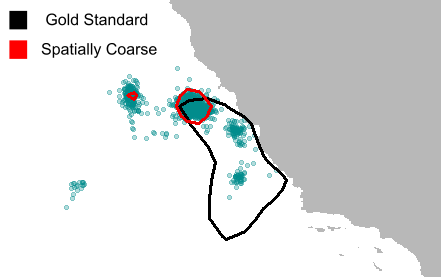
\includegraphics[width=4in]{geo_12_tmp_1_ud.png}
    \caption{Contour map comparing the 95\% utilization distribution map for the Gold Standard and 12 km resolution on September 1, 2008. Points are whales from the 12 km population.}
    \label{fig:badud}
\end{figure}
\begin{figure}[ht] \centering
    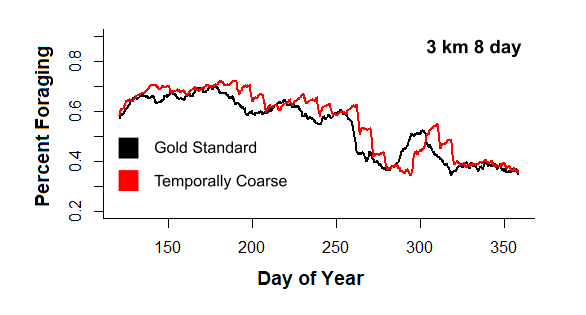
\includegraphics[width=6in]{state_geo_3_tmp_8_no_fix.png}
    \caption{Proportion of population foraging over time for the Gold Standard and 8 day resolution.}
    \label{fig:badforage}
\end{figure}

Figure \ref{fig:badud} highlights that models run on low resolution data return misleading predictions of whale positions, forecasting them to be clustered in much smaller areas than they actually are. In Figure \ref{fig:badforage}, which shows the proportion of agents foraging over time and gives a sense of population-level behaviours, it can be seen that the models inaccurately recreate whale behaviour by causing a behavioural update lag that corrects itself in jumps. Similar unrealistic predictions are expected for IBMs of other animal populations.\par

In this study, our objective is to understand how to adapt the model and data to have the IBM produce realistic predictions in spite of poor input data. To do so, we will coarsen the original ROMS data to mimic poor satellite data, then compare the results of the IBM run on the coarse data to the results of the model run on the unaltered ROMS data. From there, we will formulate model adaptations that will yield accurate results from the IBM, even when run on coarse data. \par

In the methods section, we detail the functions of the IBM, our data manipulation methods, and our proposed adaptations; as well as the metrics to compare outputs of the IBM. In the results, we describe the efficacy of our solutions, showing quantitatively and qualitatively how they improve the model output. We analyze these results, their advantages, shortcomings, and future implications in the discussion section. \par

\section{Methods}
\subsection{The ROMS Data}
Throughout the study, we utilized ROMS (Regional Ocean Modelling System) Data \cite{ROMS1} \cite{ROMS2}, with two geospatial fields: sea surface temperature (SST) and krill. The domain is located off the California coast ($32 - 42^{\circ}N$ Latitude and $116-128^{\circ}W$ Longitude) for the year 2008. \par 

The datasets are identical in shape and structure, but contain different information: SST is sea surface temperature in Celsius and krill is a relative density with values between 0 and 1.
The resolution of this data, which we will henceforth refer to as the ‘gold standard’, is 3km spatial and 1 day temporal. Imagine the environmental data to be two dimensional maps stacked vertically, one for each time interval (Figure \ref{fig:matrix}). \par

\begin{figure}[ht] \centering
    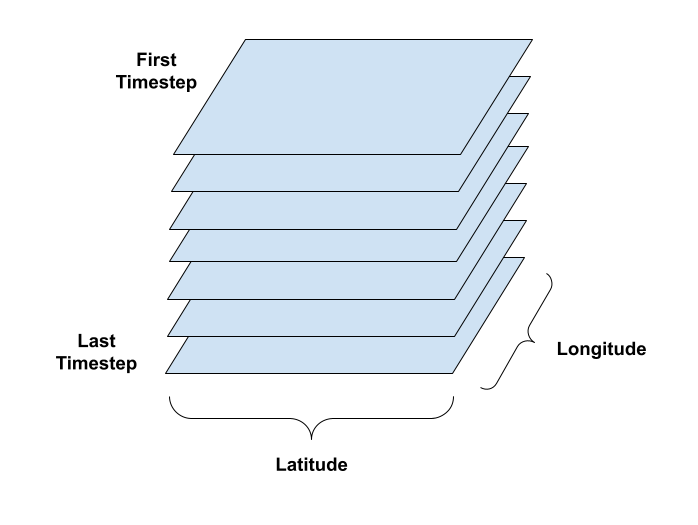
\includegraphics[width=6in]{matrixvis.png}
    \caption{Visualization of the SST and krill data as a 3-dimensional tensor.}
    \label{fig:matrix}
\end{figure}

\subsection{Description of the IBM}
Our IBM, or individual based model, takes sea surface temperature (SST) and krill data as arguments, with which whale agents interact and move realistically around the domain. As they progress through the model, the whales can occupy either a transit state ($S_1$), where they simply travel through the domain, or a foraging state ($S_2$), where they “forage” for krill; with the movement distribution of each state dictated by the step length and turning angle variables. These behavioural states are inspired by the analysis of blue whale tagging data in \cite{Bailey}. This type of model is also referred to as a “state-switching” or “semi-Markovian” model. \par

Movement updates are parametrized by step lengths and turning angles. The step lengths and turning angles for each whale are drawn from respective Gamma and Von Mises distributions with their own parameters $\mu$ and $\sigma$. Distinct distributions are defined for whales in the foraging versus transit state. On any position update, the turning angle determines at what angle from its current trajectory a whale should turn, and the step length determines how far in that direction to travel. The distributions of the step length and turning angle are also functions of the time intervals given as parameters in the model. They have moments $\mu=\text{h} \cdot 3700$, $\sigma=\text{h} \cdot 2150$ for the transiting state, and $\mu=\text{h} \cdot 1050$, $\sigma = \text{h} \cdot 970$ foraging state \cite{Bailey}, where $h$ represents the number of hours in one timestep as follows:
\begin{equation}
     \text{h}= \frac{\text{hours}/\text{day} }{ \text{steps}/\text{day} } = \frac{\text{hours}}{\text{step}}.
     \label{eqn:h}
\end{equation}
\par

% \begin{figure}[ht] \centering
%     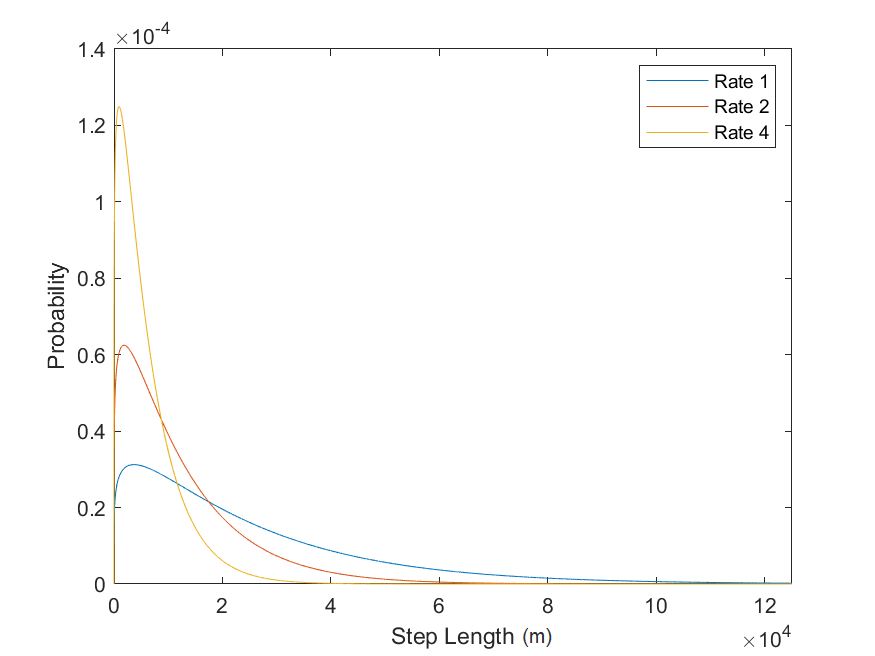
\includegraphics[width=6in]{forage_pdf.png}
%     \caption{Step length probability distributions for whales in forage state for rate 1, 2, and 4.}
%     \label{fig:steplengthforage}
% \end{figure}

% \begin{figure}[ht] \centering
%     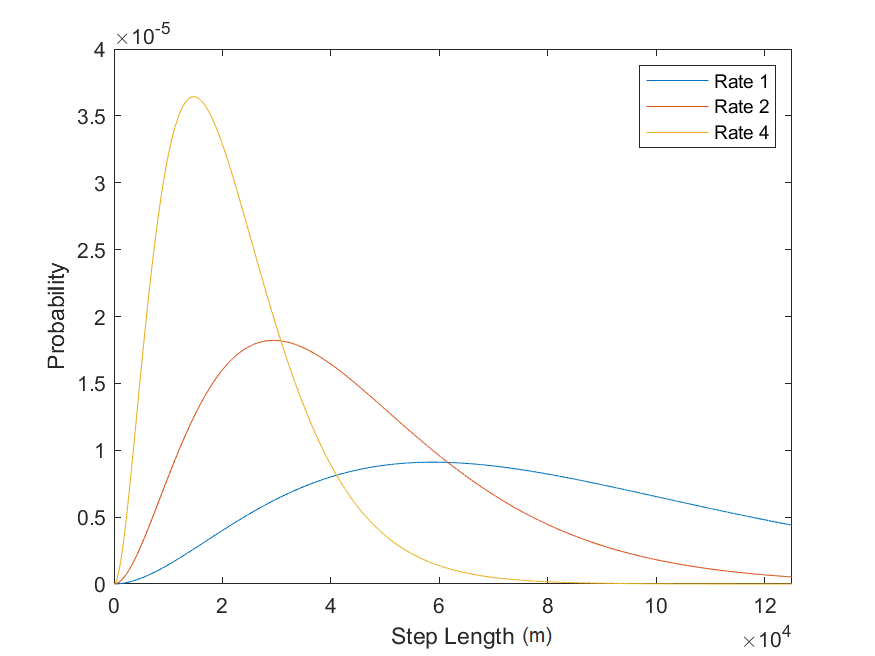
\includegraphics[width=6in]{transit_pdf.png}
%     \caption{Step length probability distributions for whales in transit state for rate 1, 2, and 4.}
%     \label{fig:steplengthtransit}
% \end{figure}

\begin{figure}[H]
	\centering
	\begin{subfigure}{3.1in}
		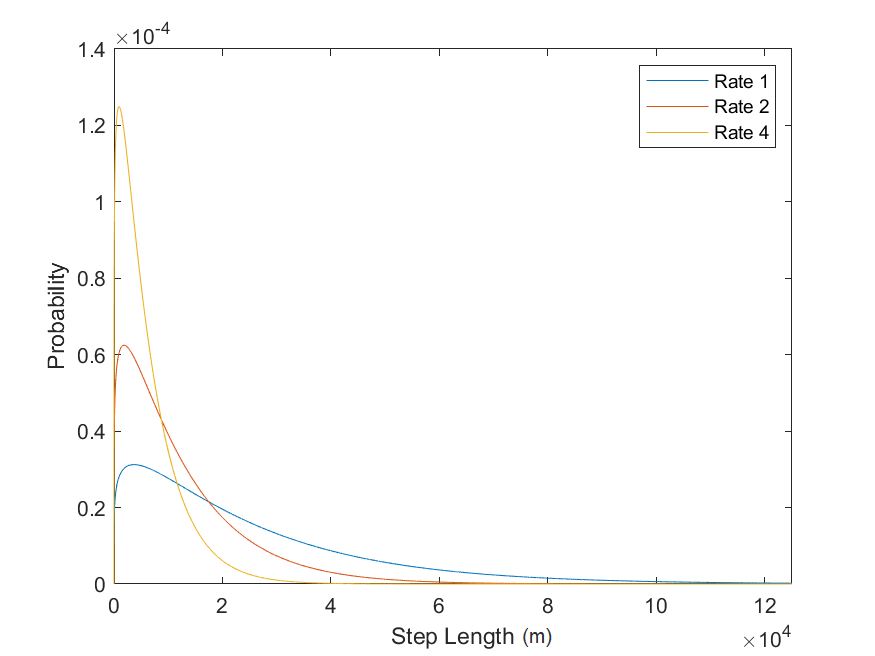
\includegraphics[width=\textwidth]{forage_pdf.png}
		\caption{Forage state}
	\end{subfigure}
%%%%%%%%%%%%%%
	\begin{subfigure}{3in}
		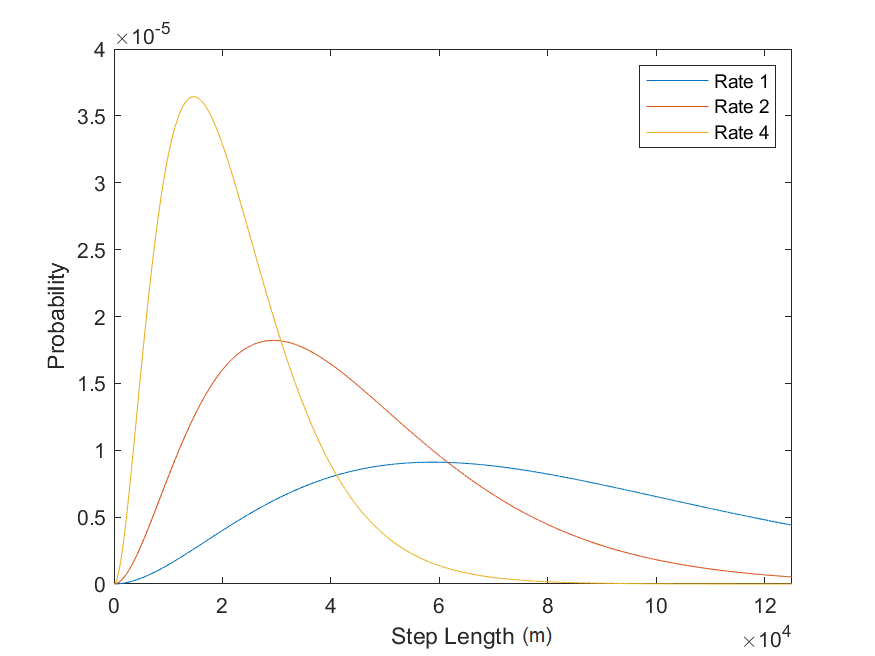
\includegraphics[width=\textwidth]{transit_pdf.png}
		\caption{Transit state}
	\end{subfigure}
    \caption{Step length probability distributions for whales in forage or transit state for rate 1, 2, and 4.}
    \label{fig:steplengthforage}    
    \label{fig:steplengthtransit}
\end{figure}

Note that, while the step length and turning angle themselves are random, the absolute direction in which the whale turns depends on its current and previous location, which form the start of the zero degree angle from which the whale will turn. Hence, the “semi-Markovian” reference. 
At every update, each individual reads its local SST and krill conditions, which influence the probability of foraging through a distribution defined by 
\begin{equation}P(S_2) = P(\text{ foraging }) = \frac 1 z \cdot (w_1\cdot P_{\text{ SST }}(\text{ foraging }|\text{ SST }) + w_2\cdot P_{\text{ krill }}(\text{ foraging }|\text{ krill }) ), \end{equation}
where $z=3$ is a normalization parameter, $w_1=1$ and $w_2=2$ are weights, and $P_{\text{ SST }}$ and $P_{\text{ krill }}$ are the respective probability distributions of foraging given SST and krill. The probability of transitioning between states can be viewed as a $2\times 2$ state-transition matrix. \par 

Lower SST and higher krill densities in a whale’s surroundings are associated with an increased likelihood of it either switching to or continuing in the foraging state (Figure \ref{fig:probkrill}).\par


\begin{figure}[H]
	\centering
	\begin{subfigure}{3.2in}
		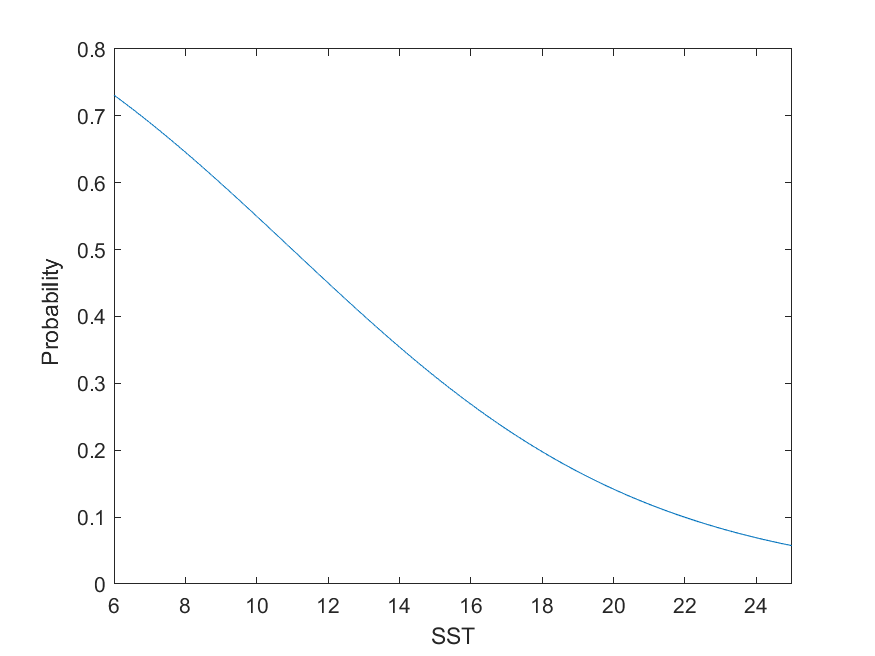
\includegraphics[width=\textwidth]{change_sst_pdf.png}
		\caption{Based on surrounding SST}
	\end{subfigure}
%%%%%%%%%%%%%%
	\begin{subfigure}{3in}
		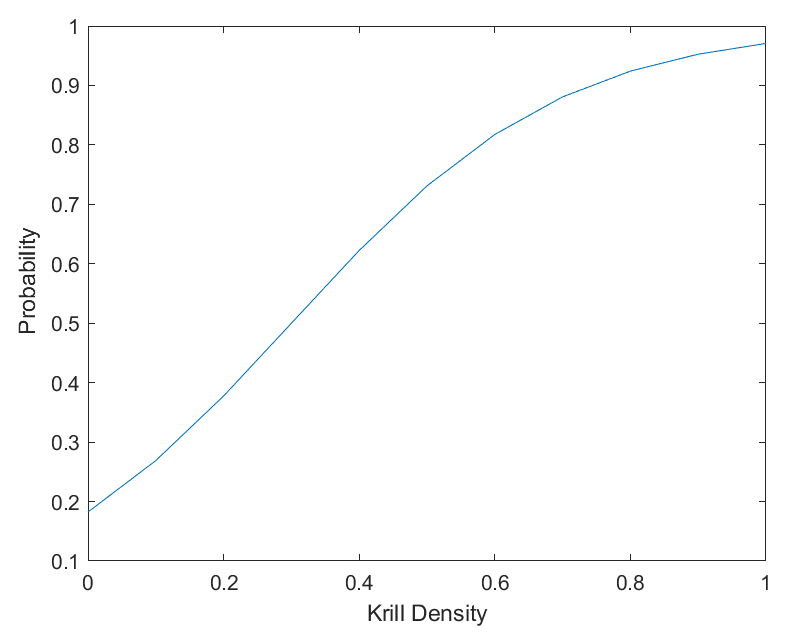
\includegraphics[width=\textwidth]{change_krill_pdf.png}
		\caption{Based on surrounding krill density}
	\end{subfigure}
    \caption{Probability of a whale foraging based on its environment.}
    \label{fig:probkrill}    
    \label{fig:probsst}
\end{figure}


% \begin{figure}[ht] \centering
%     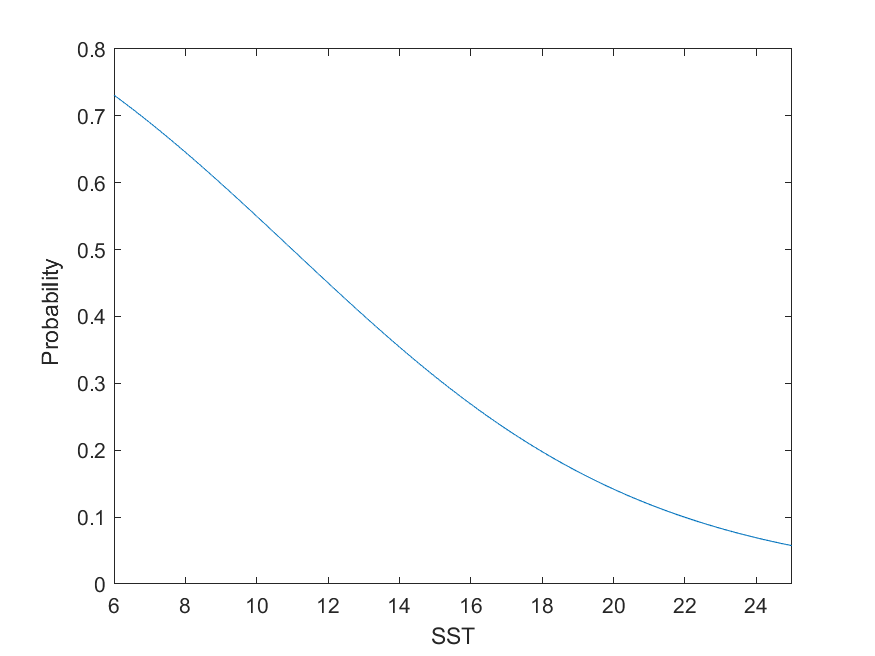
\includegraphics[width=6in]{change_sst_pdf.png}
%     \caption{Probability of a whale foraging based on surrounding SST.}
%     \label{fig:probsst}
% \end{figure}

% \begin{figure}[ht] \centering
%     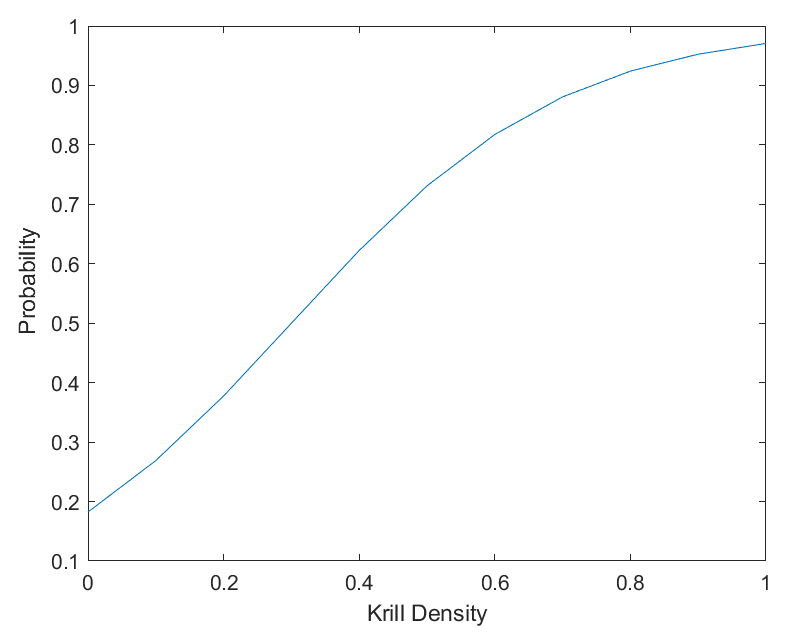
\includegraphics[width=6in]{change_krill_pdf.png}
%     \caption{Probability of a whale foraging based on surrounding krill density.}
%     \label{fig:probkrill}
% \end{figure}

To summarize the process: the IBM is initiated on May 1st in the southern portion of the domain, and at each update, the whales select a movement distance based on the distributions in Figure \ref{fig:steplengthforage} and their current location. Their foraging state is determined from their environmental conditions. This update cycle repeats until the end of the simulation, which, in this case, is the end of the year.\par

\subsection{Data Coarsening in Space and Time}
We manipulated the ROMS data to mimic the data collection shortcomings of satellites. Specifically, satellite readings are plagued by coarse spatial and temporal resolutions. These are in part due to a satellite's movement, type of readings, and presence of cloud cover. Making the data ‘bad’ in the way that satellite data is flawed required coarsening the data in space and time. \par 

Spatial coarsening of the SST and krill ROMS data was accomplished through Matlab’s \texttt{meshgrid} and \texttt{interp3} functions, which together took as input the data the original 3km spatial resolution, and returned it in lower resolutions of 6 km, 9 km, and 12 km. These coarser resolutions were selected to match available satellite data and test the limits of our methods.\par 

To make up for missing data over time, satellites tend to use moving means; thus, our temporal coarsening was accomplished through averaging the data over time. To obtain coarsened data with an $n-$day resolution, we averaged the data in every $n$ time-slices. The $n$ slices were compressed into a single slice, resulting in a total of $1/n$ times the number of original time-slices. We performed this temporal averaging for 3 days and 8 days to mimic time resolutions consistent with satellite data. \par 

\begin{figure}[ht] \centering
    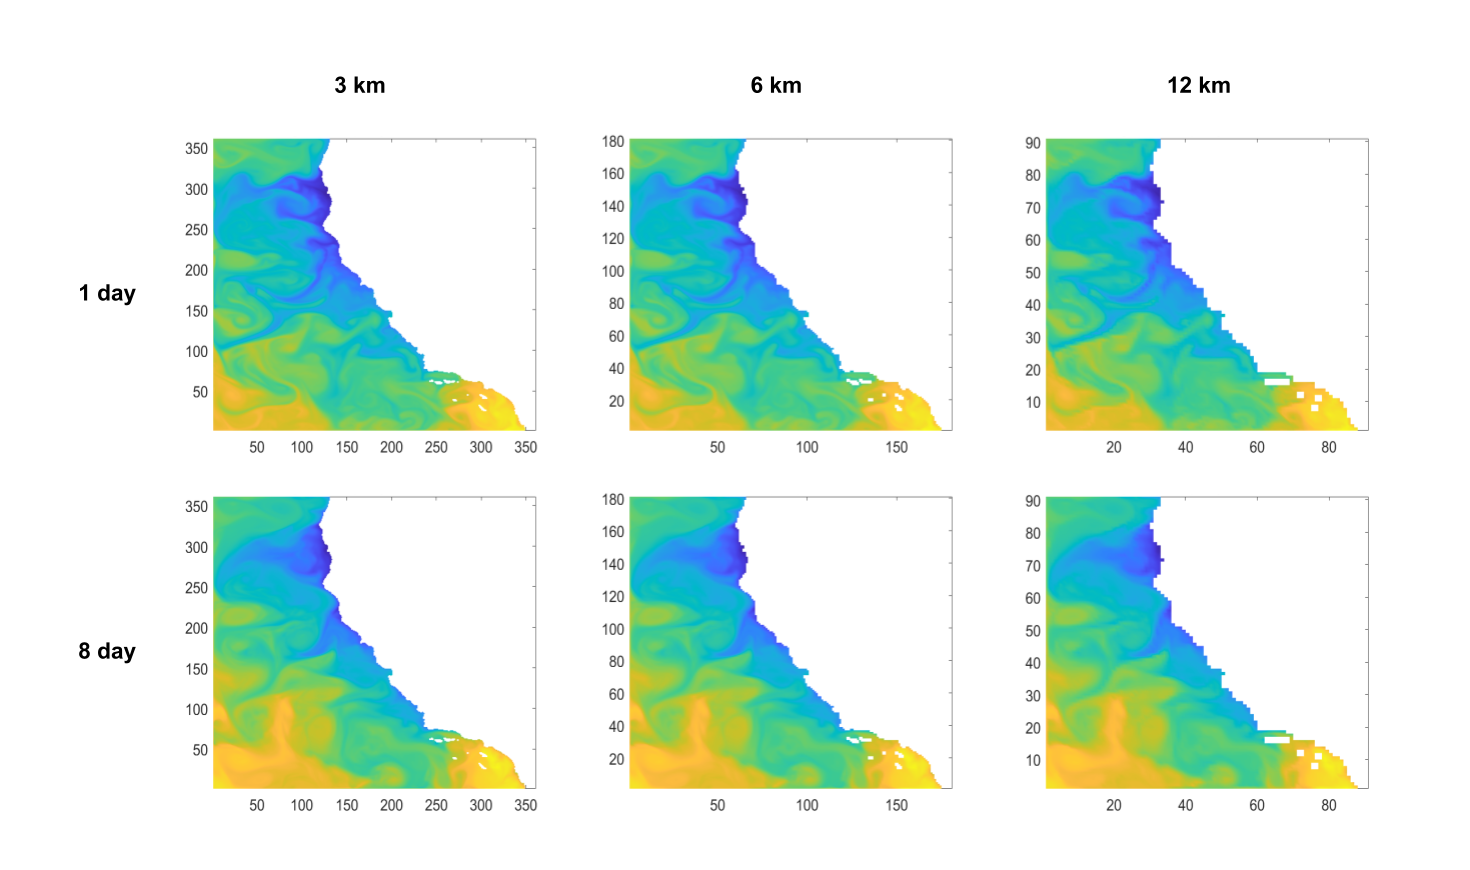
\includegraphics[width=6in]{sst_maps.png}
    \caption{SST data from September 1, 2008, coarsened temporally and spatially. The axes of each map show the number of grid cells from the bottom left corner.}
\end{figure}

Note that minor alterations to the IBM’s parameters, not mentioned because of their triviality, were required so that the model would run given the new dimensions of the data. \par

\subsection{Issues from Coarser Data}
Once we had coarsened the data, feeding it into the IBM no longer resulted in the same whale behaviour or locations as the gold standard. We note that the gold standard model uses data with 3 km, 1 day spatiotemporal resolution. Unlike many of the models based on coarser data, the gold standard results in whale locations spread over the coast and and continuous population foraging behaviour. In model iterations parametrized by the more extreme resolutions, like 12 km in space or averaged over 8 days in time, the coarse data caused the population to act completely differently. \par 

When acting based on data coarsened in space (Figure \ref{fig:badud}), the whales tended to move closer to each other as the simulation progressed, resulting in them clustering unrealistically at the coast instead of being spread over the domain. Adding temporal coarsening to the data only exacerbated this clumping effect. \par 

\begin{figure}[ht] \centering
    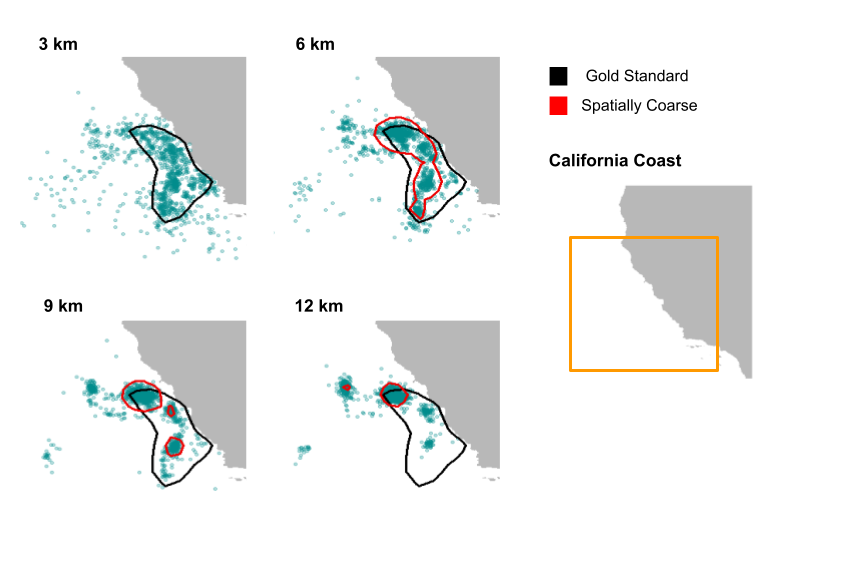
\includegraphics[width=6in]{spatial_coarsening.png}
    \caption{Zoomed in utilization distribution maps of spatially coarse data vs. the gold standard. Curves show the 95\% contour of the UDs. The full domain is shown on the right, with the regions in the left indicated by the orange box.}
    \label{fig:udfix}
\end{figure}

In addition to causing the whales to cluster over time, temporal coarsening alone also altered whale behaviour. Abrupt jumps in the percentage of whales foraging became apparent at the end of each time-slice, making the whales' feeding behaviour unrealistically stepwise for extremely coarse time (Figure\ref{fig:badforage}).\par 

\begin{figure}[ht] \centering
    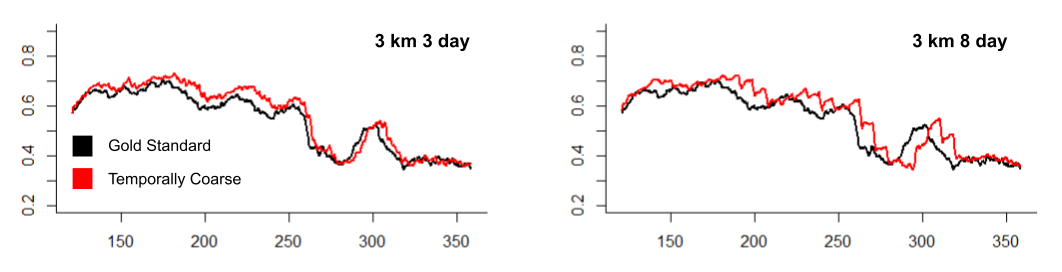
\includegraphics[width=6in]{temporal_coarsening.png}
    \caption{Percentage of population foraging over time for temporally coarse data vs. the gold standard.}
\end{figure}

These deviations from the gold standard output required that we alter the IBM or its inputs such that the IBM would continue to produce realistic results, even with poor data. \par

\subsection{Model Adaptations: Spatial}
In an effort to have the IBM running on coarse data reproduce the same movement and behavioural patterns as the gold standard IBM running on the gold standard ROMS data, we modified parts of its algorithm; in particular, we scaled the the time-steps of the IBM. \par

To mitigate the issues that arose specifically from spatially coarse data, we adjusted the rate at which the whales updated their locations and behavioural states. In the gold standard model, the whales take 4 steps per day (every 6 hours), with step length selected from a Gamma distribution with parameters $\mu_0$ and $\sigma_0$. In order to recover realistic whale movements; i.e. to have the whales move the same distance over the same amount of time, we scaled this distribution by a parameter $h$ defined in (\ref{eqn:h})
% \begin{equation} r = \frac{24}{\text{steps/day}} = \frac{\text{length of timestep}}{\text{timesteps}/\text{day}} \end{equation}
to accommodate for the increased size of grid cell caused by coarse spatial data. \par

From the gold standard model's rate of 4, we changed our rates to 1 and 2, corresponding, respectively, to time steps of 24 and 12 hours. This way, the length of the steps the whales took increased as the number of steps they took decreased \cite{Bailey}. \par

\subsection{Model Adaptations: Temporal}
To mitigate the disruption to whale behaviour caused by temporally coarse data in the IBM, our ‘fix’ was to introduce temporally finer data (when available) to the coarsened data. Our intention was to develop a methodology for handling temporally coarse input data while remaining consistent with the available satellite data. Temporally finer satellite data (e.g. 1 day, or daily) is often prohibitively sparse for IBM use due to missing data from clouds or the location of the satellite, but 8-day averages are sufficiently dense. We used this structure to our advantage and augmented the coarse data with available finer resolutions. \par

We regard the coarse data as our primary input, and the fine data as our secondary input. First, we created gaps in the coarse data by using Matlab’s \texttt{randi} function to select 30\% of the indices in the data uniformly at random. Then, to fill in the gaps in the coarse data, we replaced the randomly selected indices of the coarse data with the fine. In short, given temporally coarse data, we backed it up, or combined it with data of similarly coarse spatial, but finer temporal (1 day) resolution. For example, we might modify the 6 km 8 day coarse data by replacing 30\% of it with the finer 6 km 1 day data. \par 

Note that combining data of different resolutions in this way required some interpolation of the coarser data to the larger dimensions of the fine.\par

Before selecting 70\% as the ratio of temporally coarse data, we analyzed real GOES (Geostationary Operational Environmental Satellites) satellite data recorded from the same area of the ocean as our ROMS data. Measurements of the GOES data are gathered by the GOES Imager, a multi-channel radiometer carried aboard the satellite. This satellite data is available in 6 km spatial resolution (about 0.05 degree latitude-longitudinal resolution) and in 1, 3, 8, 14, and 30 day composites averaged in time. Satellite SST data was extracted from NOAA GOES Imager Western Hemisphere satellite and accessed via \cite{GOES}. Examples of data with few holes and many holes can respectively be found in Figure \ref{fig:satellitemanyholes}. \par
% \begin{figure}[ht] \centering
%     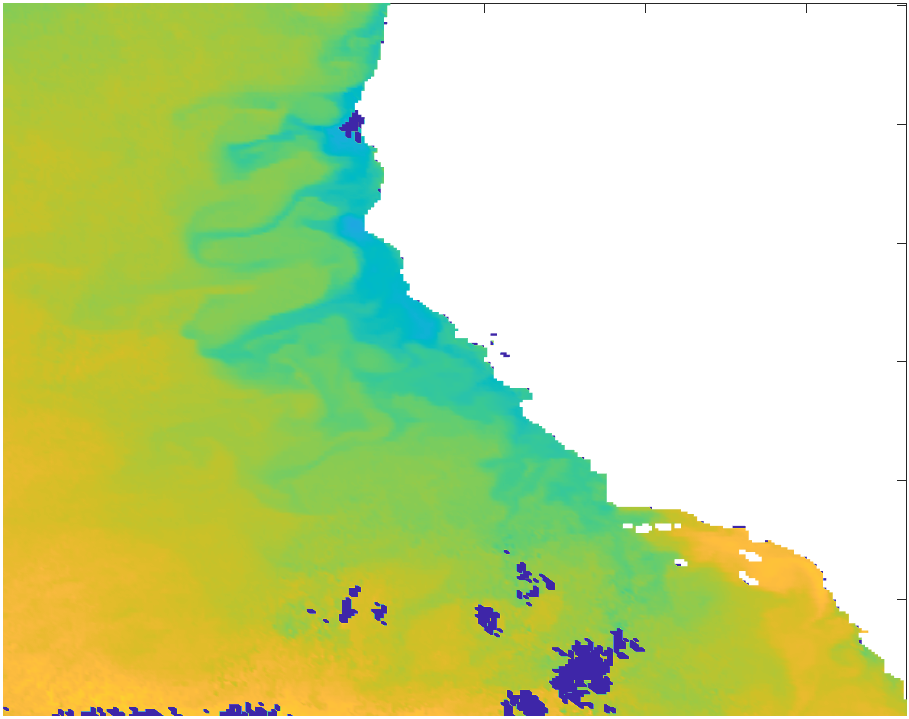
\includegraphics[width=6in]{satellite_some_holes.png}
%     \caption{SST GOES satellite data on a day with very few holes.}
%     \label{fig:satellitesomeholes}
% \end{figure}
% \begin{figure}[ht] \centering
%     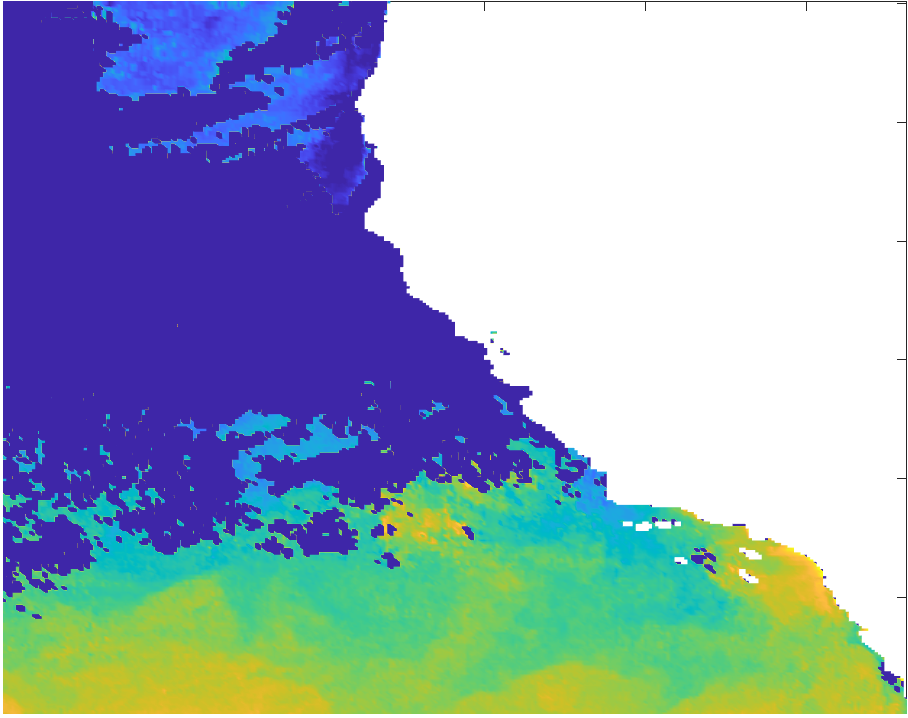
\includegraphics[width=6in]{satellite_many_holes.png}
%     \caption{SST GOES satellite data a day with many holes.}
%     \label{fig:satellitemanyholes}
% \end{figure}

\begin{figure}[H]
	\centering
	\begin{subfigure}{3.2in}
		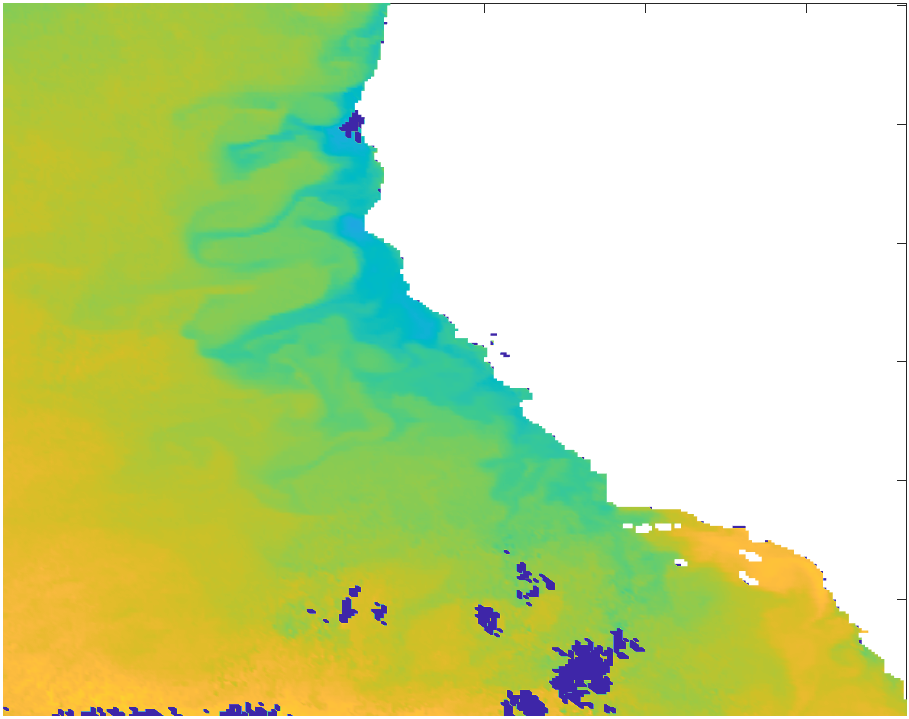
\includegraphics[width=\textwidth]{satellite_some_holes.png}
		\caption{A day with very few holes}
	\end{subfigure}
%%%%%%%%%%%%%%
	\begin{subfigure}{3.2in}
		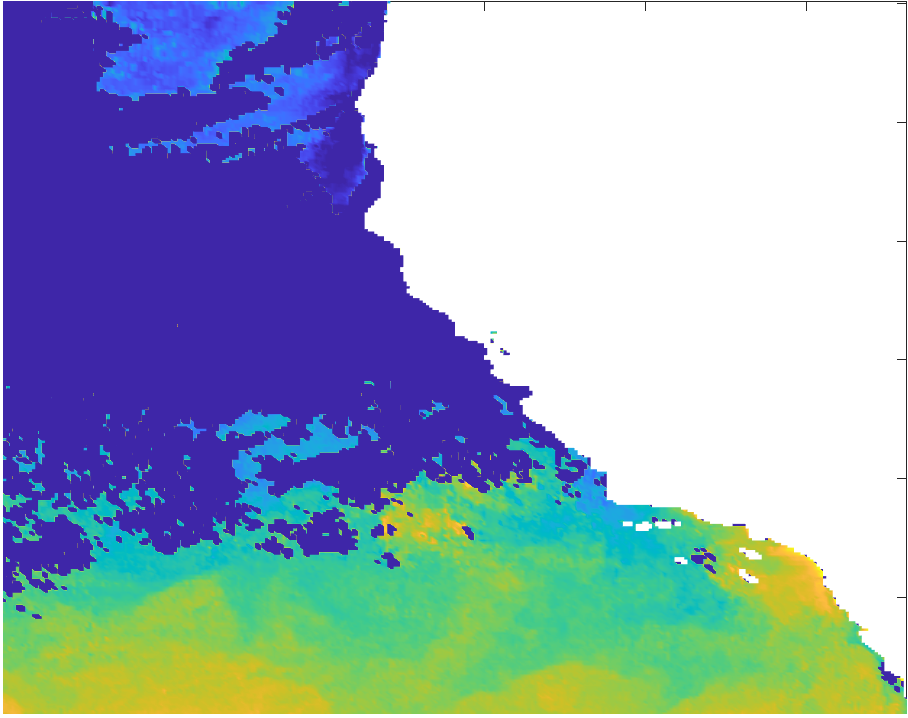
\includegraphics[width=\textwidth]{satellite_many_holes.png}
		\caption{A day with many holes}
	\end{subfigure}
    \caption{SST GOES satellite data on days with varying amounts of holes. Dark blue indicates missing data.}
    \label{fig:satellitesomeholes}    
    \label{fig:satellitemanyholes}
\end{figure}

Plotting the percentage of the data that was missing (Figure \ref{fig:goesclouds}) showed that the highest percentage of clouds at any time, for the first temporal resolution (1 day), was 80\%, with an average of 40\%. That is, on any given day, there is a wide range of data that might be missing. We also tested a range of coarse to fine ratios (i.e percentages of missing data) on our own data, and the lowest percentage of fine data that returned reasonably improved results from no fine data at all was 30\%. Thus, in what follows, we fix 30\% as the amount of fine data to introduce, and 70\% as the amount of `missing' or coarse data. The improvements will be further discussed in the Results section; see table \ref{table:allfolddelta}.  \par 

\begin{figure}[ht] \centering
    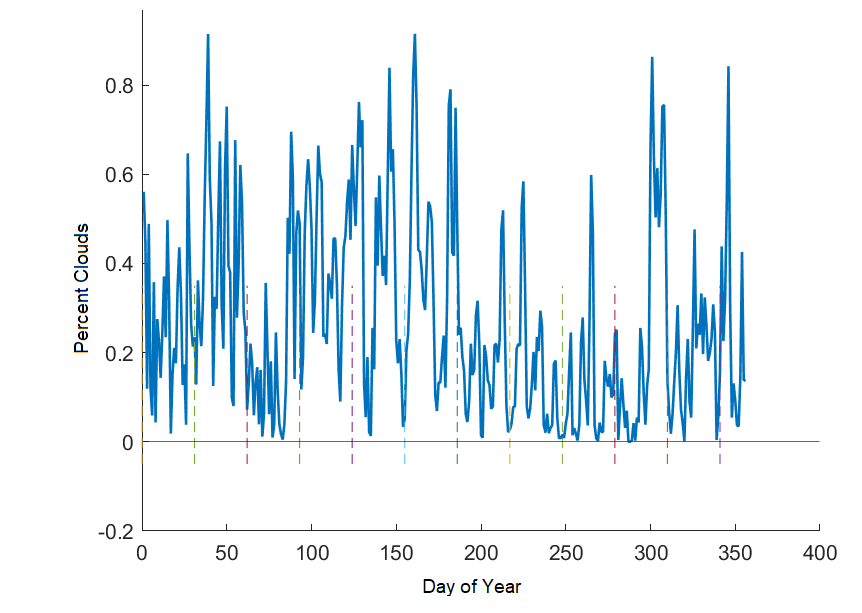
\includegraphics[width=6in]{goes_1d_cloudpercent.png}
    \caption{Percentage of the missing data for real, daily satellite GOES data. Dashed vertical lines indicate the beginning of each month.}
    \label{fig:goesclouds}
\end{figure}

\subsection{Metrics}
The behaviours that we are trying to replicate in the gold standard are the foraging behaviours over time and their habitat area. We used two established metrics to compare model outputs between the adjustments, as well as a third that we designed to be a combination of the two.\par

The L2 norm, or the Mean Square Error, was used to measure how close the whales’ foraging behaviour resulting from any of the models was to that of the gold standard model ouput. We extracted the vector of the percentage of whales foraging over time for both models and, after applying a moving mean, compared them using the L2 norm of the data. This metric provided an understanding of the foraging behaviours of the whale population through time. We define
\begin{equation}
    L2(X,X_{\text{GS}}) = \sqrt{\sum_{i=1}^n (X(i) - X_{\text{GS}}(i))^2}.
\end{equation}
Note that $X_{\text{GS}}$ represents the output produced by the gold standard model. Lower L2 norms indicate a more accurate reproduction of the gold standard outcomes, and an L2 norm of zero indicates that the models have identical foraging behaviour.  \par

Utilization distributions are probability distributions built from the point cloud of individual positions and are commonly used to understand and compare animal habitats. To quantify the accuracy of the utilization distribution produced by a given model, we used the volume intersection (‘VI’ in the \texttt{adehabitathr} R package) between the utilization distribution of the final positions of the whales from the given model versus the gold standard model. The positions were taken from September 1, 2008, a date by which the whales had had sufficient time to explore and interact with the domain. This gives a measure of how close the model output is to the gold standard in terms of whale positions. We refer to this volume as the ‘VI’. The equation for the VI integral is
\begin{equation}\text{VI}(X) = \int_x\int_y \min(\text{UD}_{X}(x,y),\text{UD}_{\text{GS}}(x,y)) dxdy \end{equation}
for model run $X$ compared to the gold standard model at all points $(x,y)$ in our domain. 

Because we are measuring overlap of the utilization distributions, a higher value indicates better model performance, with the maximum being 1. Due to the stochastic nature of the model, a VI value of 1 was not achieved even by comparing two of the same model runs from the gold standard, which returned an overlap value of around 99\%; thus, for our purposes, VI values near 0.9 are considered good. \par 
The UDs and VI values were computed using R. We formatted the final whale positions of each model, labelled by the resolution of its input data, into a dataframe, then used the \texttt{kerneloverlap} and \texttt{kernelUD} functions from the {R} (version 4.0.2) package \texttt{adehabitatHR} \cite{Rpackage} to return the VI overlap value. Our choice of setting the method argument to 'VI' gave us the computed volume of intersection between the gold standard and coarse data model outputs. \par

Finally, our own $\Delta$ metric is the combination of the L2 and VI norms: for a model outcome $X$, we defined
\begin{equation}\Delta(X) = \sqrt{\text{L2}^2(X) + (1-\text{VI}(X,X_{GS}))^2(X)}.\end{equation}
Since all efforts to adapt the model were done so to make it produce equivalent results as the gold standard when fed into the simulator, our goal was to minimize the $\Delta$ of the model; i.e. minimize the L2 and maximize the VI values. We measured the effectiveness of a model adjustment by quantifying model improvement using the fold decrease in $\Delta$ values before and after the adjustment was applied.\par

\section{Results}
\subsection{Changing Rate Counteracts Spatially Coarsened Data}
We focus first on purely spatially coarsened data, which has the same 1 day temporal resolution as the data used in the gold standard. The model run on spatially coarsened data resulted in unrealistic behaviours from the whales: resolutions lower than the gold standard of 3 km prevented the whales from exploring the entirely of the domain and caused them to move closer together as the IBM progressed. In particular, the agents ended up in clusters near the coast instead of spread over the domain. In an attempt to recreate the spread-out behaviour of the gold standard IBM, we decreased the rate at which the whales updated their locations and behavioural states. \par 

Without any temporal coarsening, adjusting the rates significantly mitigated the clustering effects of spatial coarsening on the locations of the whales. Changing the rate in the IBM caused the whales to forage in generally the same areas with coarse data as they did with the gold standard data. The utilization distributions of the whales’ positions on the date September 1, which we noted was chosen as a sufficiently advanced time in the simulation to show model- representative whale behaviours (Figure \ref{fig:udfix}), became visibly more similar to that of the gold standard. \par

\begin{table}[ht]
    \centering
    \begin{tabular}{llll}
    \toprule
     &6 km&9 km &12 km\\\hline
    Original VI &0.705 &0.480 &0.256\\
    Corrected VI& 0.710& 0.645& 0.549\\
    Fold Decrease $\Delta$& 1.617& 1.920& 1.800\\
    \toprule
    \end{tabular}
    \caption{Original and corrected VI for spatially coarsened data, with fold decrease in $\Delta$ values.}
\end{table}

\begin{figure}[ht] \centering
    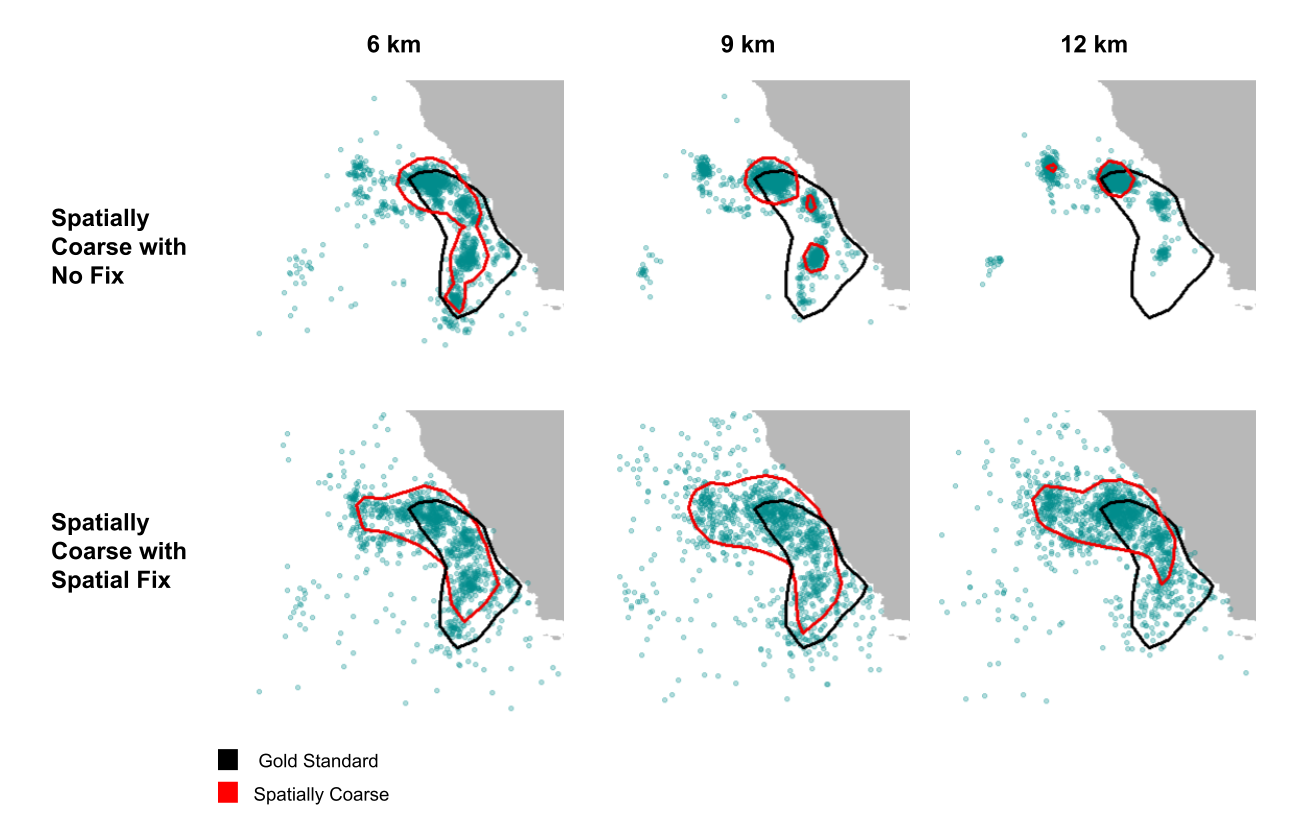
\includegraphics[width=6in]{spatial_fix.png}
    \caption{Utilization distribution maps of spatially coarsened data with and without altered rates.}
\end{figure}

The original VI values for the coarse data for 9 km, and 12 km were 0.705, 0.480, and 0.256 respectively. Recall that higher VI values, closer to the maximum of 1, are more desirable. After adjusting the rate, these values became 0.710, 0.654, and 0.549; all improvements, even to the 6 km, which shows less dramatic improvement due to already being relatively close to the gold standard. As well, before changing the rate, the $\Delta$ values were about 1.9, 2.8, and 3.0; all very high and indicative of undesirable model results that did not align with the gold standard. After changing the rate, these values reduced to 1.2, 1.4, and 1.7; at minimum a 1.6 fold decrease each, with the 9 and 12 km resolutions seeing the greatest favorable impacts. \par

\subsection{Introducing Finer Data Counteracts Temporally Coarsened Data}
We now consider purely temporally coarsened data, keeping the spatial resolution constant at 3 km. Recall that coarsening the data temporally caused issues with population-level whale foraging behaviour. For lower temporal resolutions than the gold standard’s 1 day, the whales experienced abrupt, en masse changes in foraging state, causing the percentage of whales foraging over time to look unrealistically segmented. To mitigate this effect, we introduced finer data as a replacement for 30\% of the coarse data as described in the Methods section. With the addition of the finer data, the foraging percentages were visually less step-like and numerically closer to the gold standard results. \par

\begin{table}[ht]
    \centering
    \begin{tabular}{lll}
    \toprule
    &3 day &8 day\\ \hline
    Original L2& 1.211&1.787\\
    Corrected L2& 0.772&0.935\\
    Fold Decrease $\Delta$& 1.623&2.004\\
    \bottomrule
    \end{tabular}
    \caption{L2 norms for temporally coarsened data before and after the addition of 30\% 1 day data, with fold decrease in $\Delta$ values.}
\end{table}

When naively fed temporally coarse data, the IBM results had $\Delta$ values of 1.4 and 2.0 respectively for 3 day and 8 day. These high $\Delta$ values are largely due to jump-like behaviours in the percentage of whales foraging. After replacing 30\% of the coarse data with available fine data, we found that the $\Delta$ values decreased over 1.6 fold and 2 fold, to a value near 1. Similarly, the L2 norms decreased, as desired, from 1.2 and 1.7 to 0.77 and 0.93 for the coarse temporal resolutions of 3 day and 8 day. \par 

\begin{figure}[ht] \centering
    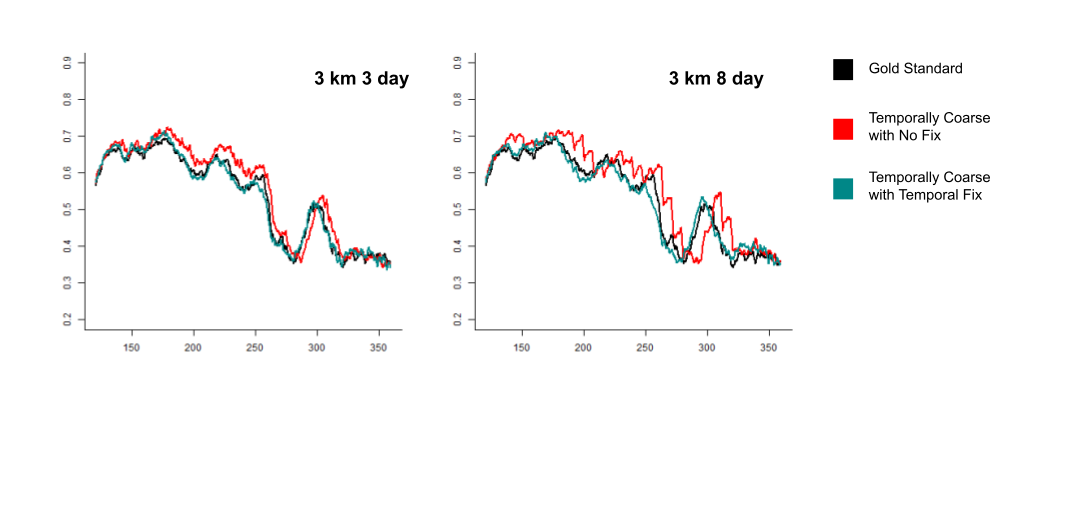
\includegraphics[width=6in]{temporal_fix.png}
    \caption{Proportion of the population foraging over time for temporally coarsened data with and without added finer data.}
\end{figure}

\subsection{Combined Spatial and Temporal Fixes}
Negative influences on whale foraging behaviours were amplified when the environmental data had both poor spatial and temporal resolutions: with no fixes, the spatiotemporally coarsened data had a minimum $\Delta$ of 3 across all resolutions. Combining the fixes by substituting available fine data, then changing model rate was successful in improving the behaviours in the combined coarseness scenario. By reducing the jumps in the number of whales in each behavioural state, and increasing the overlap between the utilization distributions of the corrected and gold standard models, we were able to decrease the $\Delta$ value to be capped at 1.6. This was at least a 2.6 fold decrease in $\Delta$s for each of the spatiotemporally coarsened datasets, greater than for any of the adjustments applied to data coarse in only one dimension. \par 

\begin{table}[ht]
    \centering
    \begin{tabular}{lllll}
    \toprule
    &3 km&6 km&9 km&12 km\\\hline
    1 day&&	1.617&	1.920	&1.800\\
    3 day&1.623&	2.963	&2.700&	3.220\\
    8 day&2.004&	3.305	&3.257&	3.770\\
    \bottomrule
    \end{tabular}
    \caption{Fold decrease in $\Delta$ for all spatiotemporal coarsening combinations.}
    \label{table:allfolddelta}
\end{table}

\begin{figure}[ht] \centering
    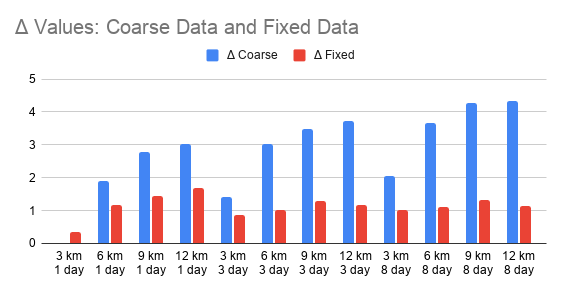
\includegraphics[width=6in]{new_old_delta_bar.png}
    \caption{Bar chart of $\Delta$ values for spatiotemporally coarse data before and after algorithm modifications.}
\end{figure}

\section{Discussion}
Our long-term goal was to run the IBM on satellite data to predict real-time locations of blue whales. However, the IBM had only been shown to produce realistic predictions on fine-scale input data. Specifically, gaps and poor resolution of SST and krill data would lead to inaccurate simulations and predictions of whale movements. To the end of mimicking this ‘bad’ data, we coarsened our data spatially and temporally. By decreasing the rate at which the whales updated their locations and introducing available fine data to the coarse data, we successfully improved, as measured by the VI, L2, and $\Delta$ metrics, the results of the IBM when running on coarse data.\par 

Of our two directions of coarsening, the first we dealt with was spatial. The lower spatial resolution (e.g. 12 km instead of the gold standard 3 k.m.), or larger grid cells, caused the whales to clump together over time instead of exploring the entire domain. We hypothesized that this was because the increased size of grid cells caused the whales to be trapped in areas of high foraging; the whales’ step lengths were too short to exit areas with high foraging probability. Since the step lengths are a function of the step rate, with larger average lengths corresponding to lower rates; by decreasing the rate at which the whales updated locations, the step length became better aligned with the spatial size of the grid cells. Larger step lengths prevented the whales from getting stuck in rich foraging locations and allowed agents to step out of a grid cell and continue to explore the domain.  For example, changing the update from 6 to 24 hours (rate 4 to rate 1) shifted the average step length of foraging from 6.3 km to 25 km. The larger average step length then allowed individuals to exit a 12 km grid cell and continue to explore the domain. \par 

Our second direction of coarsening was temporal; lower temporal resolutions were apparent in sudden changes in the percentage of whales foraging. The jump-like behaviours were due to the whales operating on old information: the coarser the temporal resolution, the more outdated the whales’ knowledge of their surroundings. Our model correction was to provide the agents with the most up to date information when possible. Adding finer data into the coarse data removed the unrealistic jumps in the whales’ behaviour and yielded population-level foraging activity that better resembled the gold standard.\par 

Our solution for temporal coarsening is particularly powerful because of its scale: we only required 30\% of the coarse data to be randomly replaced with the fine to see great improvement. Analysis of  GOES satellite data showed that the average missing data during the summer and fall, commonly due to cloud cover, is usually less than 40\% and rarely exceeds 70\%. Thus, utilizing 30\% of 1 day temporal resolution data with 70\% of temporally coarse data is a realistic quantity, and actually uses the upper bound of 70\% for the amount of missing satellite data. We introduced the fine data to the coarse data uniformly at random as the natural first step, since it did not require any assumptions about the locations or shapes of the missing data. One next step would be to target localized, perhaps even moving regions for more ‘cloud-like’ replacement.  \par 

The methods we develop here are not at all unique to blue whales; they can be applied to any individual based model in which the agents make decisions based on environmental input data. These solutions are particularly useful for models that, like ours, have inputs that are dynamic in space and time; nearly any IBM for animal movement could be similarly adapted. By incorporating finer temporal data when possible and aligning the step lengths to be of the same order as the spatial grid resolution, we believe other individual based models can be used with coarse environmental data to make predictions that are considerably more similar to those they might make with finer, more accurate data.\par 

The problem of predicting animal behaviour based on environmental conditions is an important one, especially with continually changing impacts from humans and climate change. With these results and further exploration in our suggested direction, it is our hope that it will be possible to make accurate, real-time predictions of whale positions based on satellite data.\par 

\addcontentsline{toc}{section}{References}
\printbibliography[title={References}]

\end{document}